\documentclass{standalone}
% \documentclass{article}
% \usepackage[paperwidth=10cm,paperheight=7cm]{geometry}
\usepackage{tikz}
\usetikzlibrary{calc,fit}
\usepackage{media9}
\usepackage[export]{animate}

\begin{document}
% \pagecolor{white} % Cambia el color del fondo de la página
\begin{animateinline}[autoplay,loop]{24}
    \multiframe{58}{n=1+1}{
    % \multiframe{29}{n=1+1}{
\begin{tikzpicture}
    \node[shift={(current page.center)},opacity=0.5](st) at (0,0){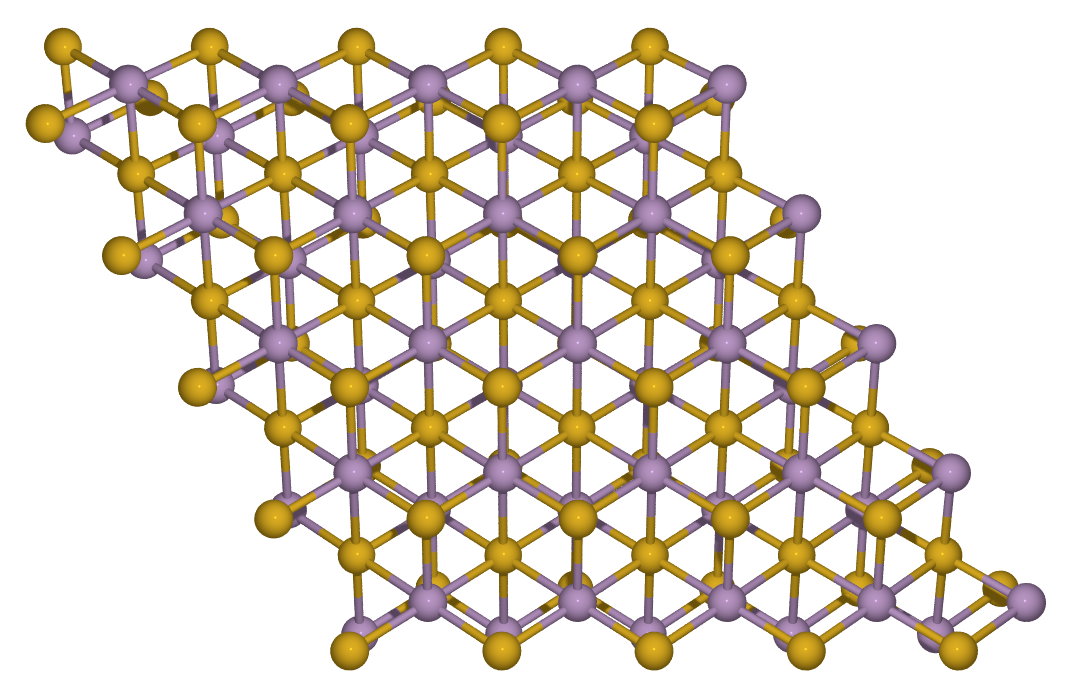
\includegraphics{./renders/Sb2Te3-uatsx-sc-0.png}};
    % \draw[blue, line width=1mm] (st.south west) rectangle (st.north east);
    \node (rect)[fit={(st.south west) (st.north east)},minimum width=40cm,minimum height=25cm] {};

\draw[blue,line width=1.5mm]([xshift=-2cm,yshift=-2.5cm]st.center)--++(6cm,0cm)--++(-3cm,5cm)--++(-6cm,0cm)--cycle;

\begin{scope}
    \clip ([xshift=-2cm,yshift=-2.5cm]st.center)--++(6cm,0cm)--++(-3cm,5cm)--++(-6cm,0cm)--cycle; 
    \node[shift={(current page.center)}](ic) at (0,0) {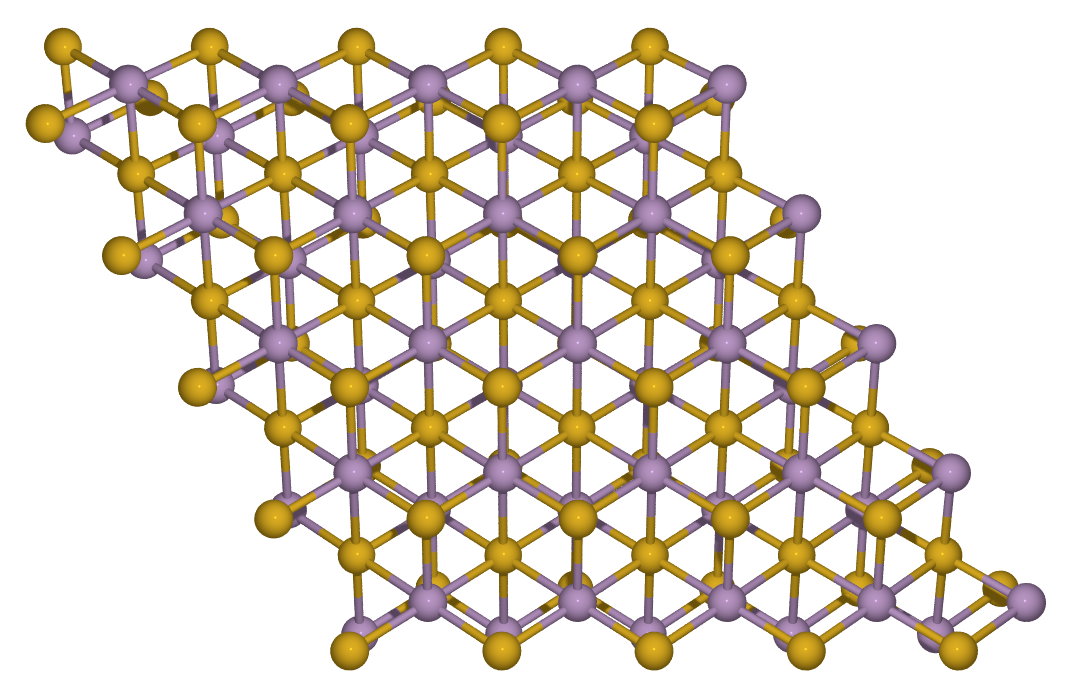
\includegraphics{./renders/Sb2Te3-uatsx-sc-0.png}};
\end{scope}

\node[anchor=north east,draw,blue,line width=1.5mm,fill opacity=0](ic0) at (rect.north east){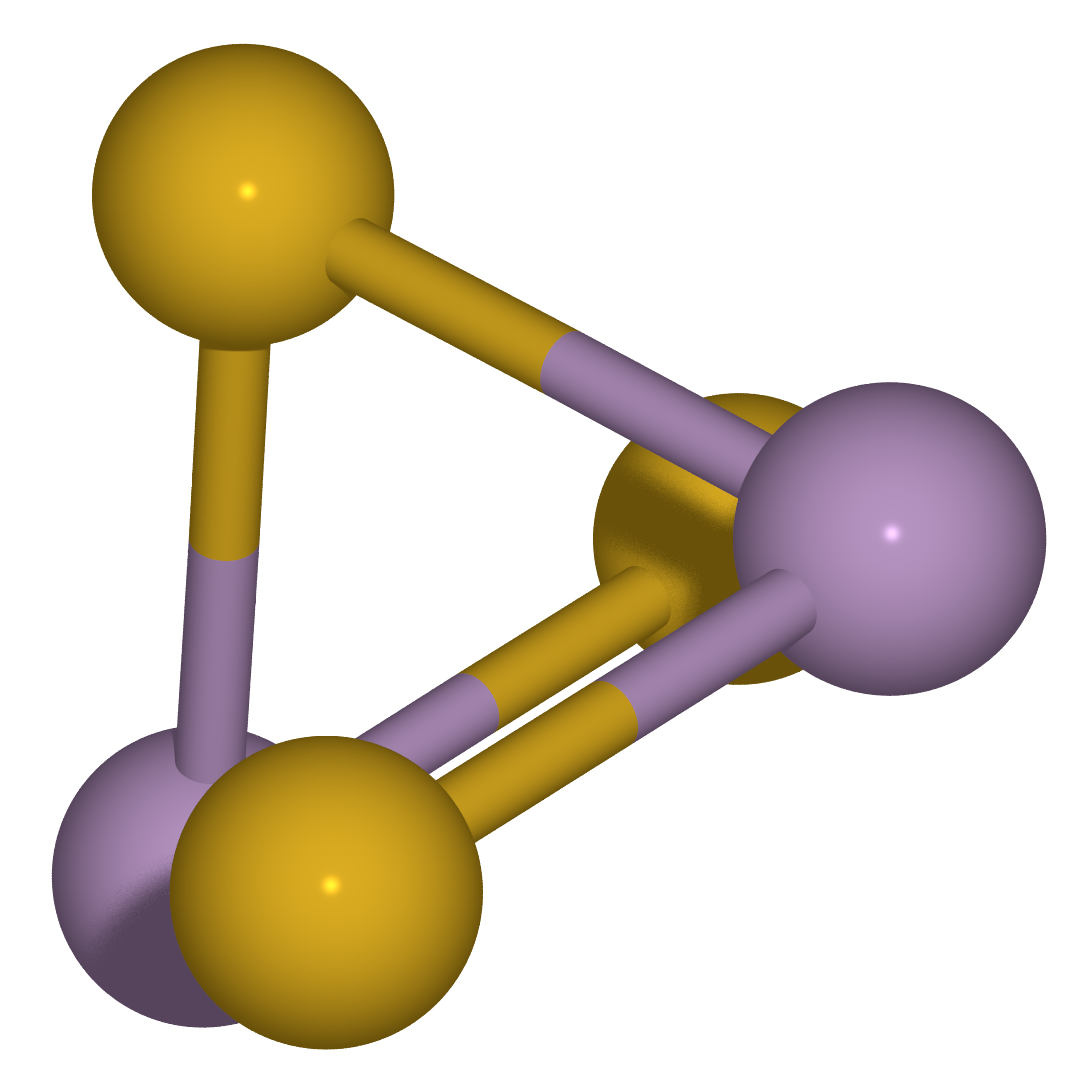
\includegraphics[width=9cm]{./renders/Sb2Te3-uatsx-uc-0.png}};

\ifnum\n<29
\node[anchor=north east](ic2) at (rect.north east) {
    \includegraphics[width=9cm]{./renders/Sb2Te3-uatsx-uc-\n.png}
};
\else
\edef\temppic{\the\numexpr 58-\n} 
\node[anchor=north east](ic2) at (rect.north east) {
    \includegraphics[width=9cm]{./renders/Sb2Te3-uatsx-uc-\temppic.png}
};
\fi

\draw[densely dashed, blue,line width=1.5mm]([xshift=4cm,yshift=-2.5cm]ic.center)--(ic0.south east);
\draw[densely dashed, blue,line width=1.5mm]([xshift=-5cm,yshift=2.5cm]ic.center)--(ic0.north west);

\end{tikzpicture}
}
\end{animateinline}
\end{document}